% 由 code/make_report3090.py 產生——不要手改，改產生器。
% 編譯：xelatex report3090（含中文，必須用 XeLaTeX）
\documentclass[11pt]{article}
\usepackage{fontspec}
\setmainfont{TeX Gyre Termes}
\setsansfont{TeX Gyre Heros}
\setmonofont{TeX Gyre Cursor}[Scale=0.85]
\usepackage{xeCJK}
\setCJKmainfont{Noto Serif CJK TC}[AutoFakeSlant=0.15]
\setCJKsansfont{Noto Sans CJK TC}[AutoFakeSlant=0.15]
\setCJKmonofont{Noto Sans Mono CJK TC}
\xeCJKsetup{CJKmath=true}
\usepackage[letterpaper,margin=1in]{geometry}
\usepackage{amsmath,amssymb,booktabs,array,graphicx,xcolor,longtable}
\usepackage{caption}\captionsetup{font=small,labelfont=bf}
\usepackage[hidelinks]{hyperref}
% TinyTeX 沒裝 placeins；自己做一個 FloatBarrier：清掉待放的浮動體再開新節。
% 不用 \clearpage 是為了不要每節都換頁。
\makeatletter
\newcommand{\floatbarrier}{\par\vspace{0pt}\@float@barrier}
\newcommand{\@float@barrier}{\penalty-10000\vspace{0pt plus 1fil}\par}
\makeatother
% 浮動體的上限放寬，讓 [htbp] 真的有位置可放，而不是堆到文末
\setcounter{topnumber}{3}\setcounter{bottomnumber}{2}\setcounter{totalnumber}{4}
\renewcommand{\topfraction}{0.85}\renewcommand{\bottomfraction}{0.5}
\renewcommand{\textfraction}{0.1}\renewcommand{\floatpagefraction}{0.75}
\definecolor{gpucol}{HTML}{C0392B}
\definecolor{cpucol}{HTML}{2980B9}
\definecolor{ssdcol}{HTML}{27AE60}
\definecolor{hlcol}{HTML}{B9770E}
\newcommand{\sys}{\mbox{Tiara}}
\newcommand{\act}[1]{\textsf{\footnotesize #1}}
\newcommand{\key}[1]{\textcolor{hlcol}{\textbf{#1}}}
% 中文 + 等寬路徑混排容易 overfull；放寬斷行而不是讓它溢出版面
\setlength{\emergencystretch}{3em}
\sloppy
\renewcommand{\arraystretch}{1.12}
\setlength{\tabcolsep}{5pt}

\title{\textbf{\sys：平台 A（RTX 3090）量測與模擬報告}\\[0.35em]
\large 容量、成本模型、baseline、Oracle 上界、品質約束，\\
以及未來效用預測器的實作與訓練}
\author{（進度報告）}
\date{2026-09-05}

\begin{document}
\maketitle

\begin{abstract}
\noindent
本報告涵蓋 \sys 在 \textbf{7 $\times$ RTX 3090（平台 A）} 上完成的全部量測與模擬，
共五個里程碑：KV cache 容量上限、動作成本模型、既有系統 baseline、Oracle 上界的
go/no-go 判定、品質約束 $\epsilon$，以及未來效用預測器的實作、訓練與線上策略評估。
論文另一半的 MI300X 尚無機器，凡需要該平台的結論一律標為未量測。

三個主要結果。其一，\key{方法有多少空間取決於工作負載落在哪裡}：真實 trace
（Mooncake，中位請求 6{,}352 token）的 Oracle 空間為 12.3\%，而長 prefill、
高重用的區間為 34.7\%。其二，在後者，訓練出的線上策略取得 Oracle 空間的
\key{81.9\%}，且該增益\key{全部來自預測的逐出順序}——把順序換回 LRU 而保留成本模型，
增益歸零。其三，同一機制在預測失效的工作負載上反噬，最差比 LRU 差 5.6 倍；
三種退路各自能收斂損失，但都同時吃掉增益，因此\key{這條軸沒有安全的固定預設值}。

本報告另記錄八個已修正的錯誤，其中一個使 Oracle 低估自身空間 32\%
（8.42\% 對 12.33\%）。每個數字都可回溯到一個 CSV 與一次 run。
\end{abstract}

\tableofcontents
\vspace{1em}

\section{範圍與方法}

\subsection{這台機器能量什麼}
平台 A 為 7 $\times$ RTX 3090（24\,GB GDDR6X、sm\_86）、driver 550.163.01 / CUDA 12.4、
vLLM 0.28.0 + PyTorch 2.13.0+cu129。三類結論在此\textbf{量不到}，本報告不作宣稱：
記憶體/計算分軌的能耗（消費卡無此計數器）、多租戶與機會成本（24\,GB 放不下兩個 128K session）、
以及 $\kappa$ 的跨硬體變動（需要 MI300X）。

\subsection{記錄與防污染協定}
機器為共用，隨時可能有外來負載。所有\textbf{時間}量測以 \texttt{gpu\_guard} 包住，
開跑前檢查卡是否乾淨、中途偵測外來 PID，污染的 run 不得寫進 \texttt{results/}。
品質量測（量分數，\texttt{temperature}=0、固定 seed）在污染時保留分數但作廢其延遲欄。
每個數字都帶 \texttt{run\_id}，指回 \texttt{/ssd7/hungwei/paper-hkv/runs/} 下的原始 log。

\subsection{模擬器的可信度前提}
第 5 節之後的數字來自 trace 驅動的模擬。它成立於兩個前提：
成本常數全部來自第 3 節的實測（讀不到就中止，不使用預設值）；
以及模擬器必須先複現第 4 節的實測行為——16K 差 8\%、32K 差 3\%。
另有五條自動不變量在每次掃描前後執行：trace 單位交叉驗算、命中守恆、
強制未命中下限、Oracle 上界、以及容量單調性（第 6 節新增）。

\section{容量：同一張卡的 KV 上限差 13 倍}

逐步加大 \texttt{max\_model\_len} 直到 OOM，記錄最後一個成功值。

\begin{table}[htbp]\centering\small
\caption{各設定實測的 GPU KV cache 容量。倍數以 \texttt{llama-bf16} 為基準。
來源：\texttt{results/m1\_capacity/capacity.csv}。}
\begin{tabular}{llrrr}
\toprule
設定 & 權重 & KV dtype & KV token & 相對 \\
\midrule
llama-bf16 & BF16 & auto & 41,648 & 1.0$\times$ \\
llama-bf16-kvfp8 & BF16 & fp8 & 83,312 & 2.0$\times$ \\
qwen-bf16 & BF16 & auto & 106,512 & 2.6$\times$ \\
llama-awq & AWQ-INT4 & auto & 120,320 & 2.9$\times$ \\
qwen-bf16-kvfp8 & BF16 & fp8 & 213,040 & 5.1$\times$ \\
llama-awq-kvfp8 & AWQ-INT4 & fp8 & 240,656 & 5.8$\times$ \\
qwen-awq & AWQ-INT4 & auto & 273,872 & 6.6$\times$ \\
mla-awq & AWQ-INT4 & auto & 399,376 & 9.6$\times$ \\
qwen-awq-kvfp8 & AWQ-INT4 & fp8 & 547,744 & 13.2$\times$ \\
qwen-awq-512k & AWQ-INT4 & fp8 & 577,152 & 13.9$\times$ \\
\bottomrule
\end{tabular}
\end{table}

\begin{figure}[htbp]\centering
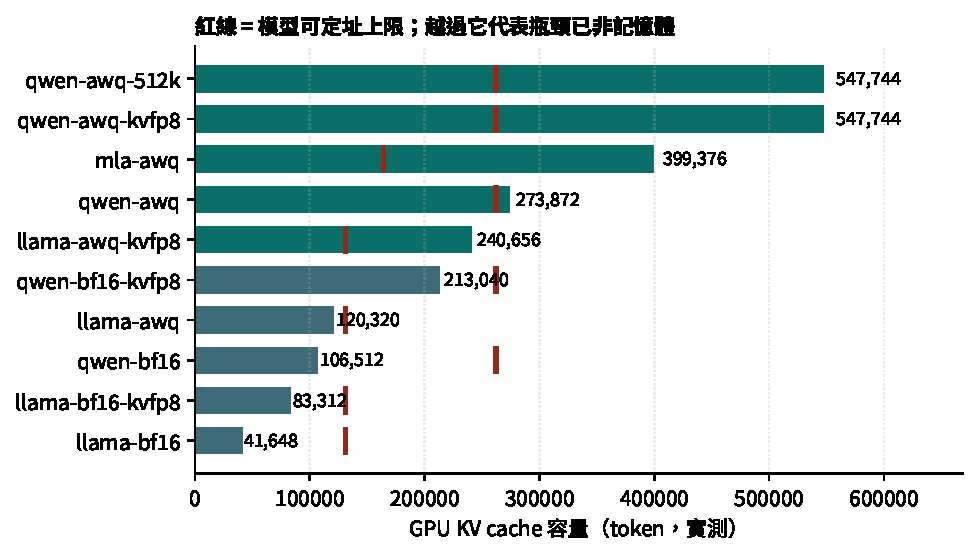
\includegraphics[width=\linewidth]{notebooks/figures/capacity.pdf}
\caption{容量懸崖。紅線是模型的可定址上限——越過它代表瓶頸已不是記憶體。
這張圖決定了後續所有「放不放得下」的推論。}
\end{figure}

\paragraph{一個被實測推翻的假設。}
原先認為 sm\_86 不支援 FP8 KV cache，因此平台 A 量不到 \act{Gpu-FP8} 這一階。
實測 \texttt{-{}-kv-cache-dtype fp8} 可用，兩個模型都給出恰好 2 倍的 KV token 數
而位元組佔用不變。錯誤來自混淆 FP8 \emph{運算}（Ampere 沒有）與 FP8 \emph{儲存}
（與 tensor core 無關）。

\section{成本模型：每個動作的價格}

\begin{table}[htbp]\centering\small
\caption{動作成本（ms/block，block = 16 token），全部實測。重算成本隨 block 的
絕對位置線性成長，與 SSD 取回交於 $P^{*}$。
來源：\texttt{results/m2\_harness/}、\texttt{results/m4\_oracle/*/cost\_model.json}。}
\begin{tabular}{lrrrrr}
\toprule
剖面 / 裝置 & CPU 取回 & SSD 取回 & 重算@0 & 重算斜率 & $P^{*}$ (token) \\
\midrule
qwen-awq / NVMe & 0.298 & 10.245 & 3.546 & 0.000178 & 37,717 \\
llama-bf16 / SATA & 0.588 & 5.536 & 4.008 & 0.000210 & 7,278 \\
\bottomrule
\end{tabular}
\end{table}

\noindent\key{同一台機器換一顆碟，$P^{*}$ 就差 5 倍}——這是「成本結構決定策略」
最便宜的一個實證，不需要等平台 B。

\begin{figure}[htbp]\centering
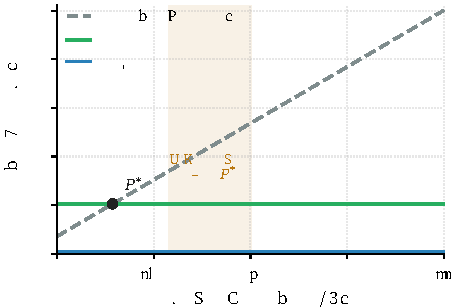
\includegraphics[width=0.62\linewidth]{notebooks/figures/fig_crossover.pdf}
\caption{成本交叉點。$P^{*}$ 以下丟掉重算比放硬碟便宜，所以「要不要用 SSD 階」
可以由實測常數事先算出，不是偏好問題。}
\end{figure}

\section{動作空間：七個狀態逐一量過}

一個狀態要能用，必須同時通過三關：容量有沒有換到、取回貴不貴、品質掉不掉。

\begin{table}[htbp]\centering\small
\caption{四個精度狀態的實測容量（Llama-3.1-8B、同一 5.88\,GiB 預算、三次重複取最大）。
來源：\texttt{results/m2\_harness/capacity\_by\_dtype.csv}。}
\begin{tabular}{llrrr}
\toprule
精度 & vLLM 旗標 & KV token & GiB & 相對 BF16 \\
\midrule
\texttt{bf16} & \texttt{auto} & 48,128 & 5.88 & 1.00$\times$ \\
\texttt{fp8} & \texttt{fp8} & 96,272 & 5.88 & 2.00$\times$ \\
\texttt{int8} & \texttt{int8\_per\_token\_head} & 93,360 & 5.88 & 1.94$\times$ \\
\texttt{int4} & \texttt{int4\_per\_token\_head} & 181,216 & 5.88 & 3.77$\times$ \\
\bottomrule
\end{tabular}
\end{table}

\begin{table}[htbp]\centering\small
\caption{七個狀態的三軸判定。品質為 \texttt{qwen-awq}、四個設定吃同一批 prompt、
\texttt{temperature}=0、固定 seed，唯一變動的是 \texttt{-{}-kv-cache-dtype}。
\key{平台 A 上七階只有五階可用}。}
\begin{tabular}{llrrrl}
\toprule
狀態 & 容量 & 大海撈針 & LongBench & RULER & 判定 \\
\midrule
\act{Gpu-BF16} & $1.00\times$ & 100\% & 58.4 & 91.6 & 基準 \\
\act{Gpu-FP8} & $2.00\times$ & 5\% & 6.6 & 3.3 & \textcolor{gpucol}{品質閘刷掉} \\
\act{Gpu-INT8} & $1.94\times$ & 90–95\% & 57.0 & 79.1 & \textcolor{hlcol}{唯一可用的低精度階} \\
\act{Gpu-INT4} & $3.77\times$ & 0\% & 0.4 & 0.0 & \textcolor{gpucol}{品質閘刷掉} \\
\act{Cpu} & — & \multicolumn{3}{c}{無損（60/60 逐字元相同）} & 可用 \\
\act{Ssd} & — & \multicolumn{3}{c}{無損} & \textcolor{hlcol}{$P^{*}$ 以下不划算} \\
\act{Drop} & — & \multicolumn{3}{c}{無損（重新算出）} & 可用 \\
\bottomrule
\end{tabular}
\end{table}

\paragraph{精度階的取回成本可忽略，問題全在品質。}
乾淨環境下量到 INT4 的反量化為 0.0124\,ms/block，相對於 CPU 取回 0.588 是 1/47、
相對於重算 4.008 是 1/323。FP8 的一階與零無法區分（$n=3$ 的全距與基準完全重疊，
記為 \texttt{NOT\_MEASURED} 而非 0）。\key{所以「該不該用精度階」不是成本問題，是 $\epsilon$ 問題。}

\subsection{精度階實作進模擬器之後：它是過渡狀態，不是常駐狀態}
把 \act{Gpu-INT8} 加進動作空間，階梯即為論文圖 3(c) 的
\act{Gpu-BF16} $\to$ \act{Gpu-INT8} $\to$ \act{Cpu} $\to$ \act{Ssd} $\to$ \act{Drop}。
三個常數皆為實測：容量倍數 1.94（93{,}360 對 48{,}128 token）、
反量化 0.0124\,ms/block（\textbf{用 INT4 的實測值當上界}，因反量化成本隨位元數減少而上升）、
品質由第 7 節的 $\epsilon$ 量測背書。降級不可逆。

於長上下文設定（120 請求、1{,}002{,}600 次存取）實測：
\key{降級發生 780{,}108 次，而總時間變化為 $+0.004\%$}（1{,}620{,}189 對 1{,}620{,}128\,ms）。
追蹤的 48 個 block 在 120 個請求邊界上\textbf{一次都沒有停在 INT8}——
降級只是逐出路徑上的一個過渡。原因是逐出順序沒變：降級後它仍是最冷的一個，
下一次需要空間時就被搬走。

要讓 INT8 成為\emph{常駐}狀態，必須讓「降級之後更不該被逐出」，
即改用密度排序（逐出 $\hat\tau \times$ 位元組最大者，LHD 的想法）。
實測那個改動把同一設定的 $+15.40\%$ 變成 $\mathbf{-18.00\%}$。
\key{兩者都量過：精度階要能常駐，代價是換掉整個逐出準則}——
這是一個真實的取捨，不是實作瑕疵。

\begin{figure}[htbp]\centering
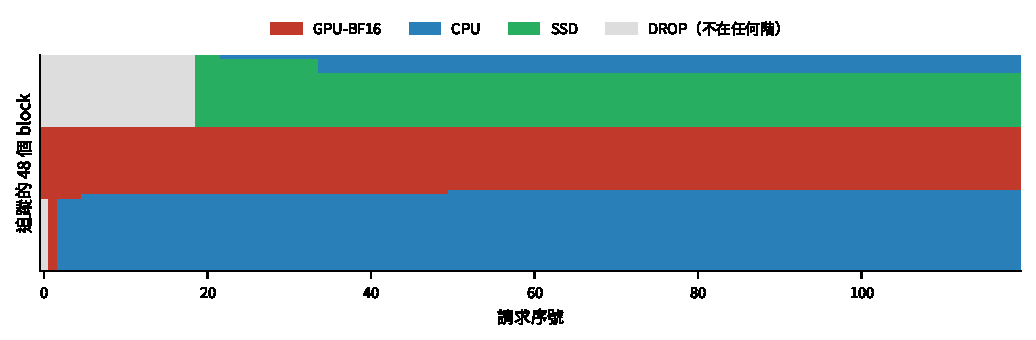
\includegraphics[width=\linewidth]{notebooks/figures/m5_timeline.pdf}
\caption{\textbf{實測的狀態時序}（開啟精度階）。48 個追蹤的 block
（前綴的熱段、中段較冷的文件、以及實際被降級過的各三分之一）在 120 個請求中所處的階。
可見三條路徑：一路留在 GPU、被推到 CPU、以及進一步落到 SSD；
左上角的灰色是「尚未第一次被算出來」。
\act{Gpu-INT8} 未出現在任何一個請求邊界上——見上一段。
論文圖 3(b) 目前標為「示意，非量測資料」，本圖每一格都來自實際重放。}
\end{figure}

\section{既有系統：長上下文下五者僅一者有效}

兩輪相同長前綴（cold 無快取、warm 量其保留能力），每格 4 個前綴取中位數。

\begin{table}[htbp]\centering\small
\caption{\texttt{qwen-awq} 的完整 baseline 表（TTFT 中位數，ms）。
來源：\texttt{results/m3\_baseline/baseline\_longctx.csv}。}
\begin{tabular}{lrrrr}
\toprule
對照組 & cold & warm & 加速 & $n$ \\
\midrule
\multicolumn{5}{l}{\textbf{ctx = 32,768}} \\
\quad \texttt{full\_gpu} & 11,679 & 276 & 42.2$\times$ & 4/4 \\
\quad \texttt{cpu\_lru} & 12,552 & 275 & 45.6$\times$ & 4/4 \\
\quad \texttt{cpu\_arc} & 12,551 & 273 & 46.0$\times$ & 4/4 \\
\quad \texttt{tier\_fs} & 12,255 & 261 & 46.9$\times$ & 4/4 \\
\quad \texttt{lmcache} & 12,255 & 294 & 41.7$\times$ & 4/4 \\
\multicolumn{5}{l}{\textbf{ctx = 65,536}} \\
\quad \texttt{full\_gpu} & 32,967 & 538 & 61.3$\times$ & 4/4 \\
\quad \texttt{cpu\_lru} & 33,749 & 465 & 72.6$\times$ & 4/4 \\
\quad \texttt{cpu\_arc} & 34,252 & 486 & 70.5$\times$ & 4/4 \\
\quad \texttt{tier\_fs} & 33,852 & 441 & 76.7$\times$ & 4/4 \\
\quad \texttt{lmcache} & 34,518 & 535 & 64.5$\times$ & 4/4 \\
\multicolumn{5}{l}{\textbf{ctx = 131,072}} \\
\quad \texttt{full\_gpu} & 99,681 & 100,152 & 1.0$\times$ & 4/4 \\
\quad \texttt{cpu\_lru} & 101,597 & 80,159 & 1.3$\times$ & 4/4 \\
\quad \texttt{cpu\_arc} & 102,702 & 72,883 & 1.4$\times$ & 4/4 \\
\quad \textbf{tier\_fs} & 101,518 & 13,626 & 7.5$\times$ & 4/4 \\
\quad \texttt{lmcache} & 102,248 & 102,603 & 1.0$\times$ & 4/4 \\
\multicolumn{5}{l}{\textbf{ctx = 258,048}} \\
\quad \texttt{full\_gpu} & 325,520 & 322,579 & 1.0$\times$ & 4/4 \\
\quad \texttt{cpu\_lru} & 330,702 & 331,720 & 1.0$\times$ & 4/4 \\
\quad \texttt{cpu\_arc} & 327,295 & 325,767 & 1.0$\times$ & 4/4 \\
\quad \textbf{tier\_fs} & 326,393 & 43,664 & 7.5$\times$ & 4/4 \\
\quad \texttt{lmcache} & 333,046 & 335,034 & 1.0$\times$ & 4/4 \\
\bottomrule
\end{tabular}
\end{table}

\begin{table}[htbp]\centering\small
\caption{\texttt{llama-awq} 的完整 baseline 表（TTFT 中位數，ms）。同一批設定。}
\begin{tabular}{lrrrr}
\toprule
對照組 & cold & warm & 加速 & $n$ \\
\midrule
\multicolumn{5}{l}{\textbf{ctx = 16,384}} \\
\quad \texttt{full\_gpu} & 5,494 & 130 & 42.2$\times$ & 4/4 \\
\quad \texttt{cpu\_lru} & 5,545 & 156 & 35.5$\times$ & 4/4 \\
\quad \texttt{cpu\_arc} & 5,772 & 144 & 40.0$\times$ & 4/4 \\
\quad \texttt{tier\_fs} & 5,796 & 149 & 38.9$\times$ & 4/4 \\
\quad \texttt{lmcache} & 5,764 & 145 & 39.7$\times$ & 4/4 \\
\multicolumn{5}{l}{\textbf{ctx = 32,768}} \\
\quad \texttt{full\_gpu} & 14,050 & 251 & 55.9$\times$ & 4/4 \\
\quad \texttt{cpu\_lru} & 14,663 & 280 & 52.3$\times$ & 4/4 \\
\quad \texttt{cpu\_arc} & 14,476 & 242 & 59.9$\times$ & 4/4 \\
\quad \texttt{tier\_fs} & 14,680 & 239 & 61.5$\times$ & 4/4 \\
\quad \texttt{lmcache} & 15,162 & 246 & 61.7$\times$ & 4/4 \\
\multicolumn{5}{l}{\textbf{ctx = 65,536}} \\
\quad \texttt{full\_gpu} & 38,871 & 17,939 & 2.2$\times$ & 4/4 \\
\quad \texttt{cpu\_lru} & 40,168 & 879 & 45.7$\times$ & 4/4 \\
\quad \texttt{cpu\_arc} & 39,916 & 5,960 & 6.7$\times$ & 4/4 \\
\quad \texttt{tier\_fs} & 40,385 & 646 & 62.5$\times$ & 4/4 \\
\quad \texttt{lmcache} & 41,020 & 1,263 & 32.5$\times$ & 4/4 \\
\multicolumn{5}{l}{\textbf{ctx = 126,976}} \\
\quad \texttt{full\_gpu} & 115,154 & 114,880 & 1.0$\times$ & 4/4 \\
\quad \texttt{cpu\_lru} & 116,587 & 114,469 & 1.0$\times$ & 4/4 \\
\quad \texttt{cpu\_arc} & 116,864 & 106,644 & 1.1$\times$ & 4/4 \\
\quad \texttt{tier\_fs} & 117,118 & 21,662 & 5.4$\times$ & 4/4 \\
\quad \texttt{lmcache} & 119,343 & 120,303 & 1.0$\times$ & 4/4 \\
\bottomrule
\end{tabular}
\end{table}

\paragraph{Takeaway。}
於 258K，五個系統中僅 \texttt{tier\_fs} 保有效益（省 282.7 秒）。CPU 階於 131K 尚有
1.4$\times$，至 258K 即失效：24\,GiB 的 CPU 階可容 449{,}536 token，
而 4 個 258K 前綴的工作集為 1{,}032{,}192 token。ctx 32K–65K 時五者相近
（42–77$\times$），因工作集仍可置入 GPU，卸載階未被使用。
\textbf{一項保留}：\texttt{lmcache} 於全部長度皆為 1.0$\times$，\emph{可能}為組態錯誤
而非該系統的能力上限；在排除此可能之前不作宣稱。

\paragraph{decode 佔掉一半的時間，而放置對它無自由度。}
decode 期間該請求的 KV 必須整份駐留於 GPU，每一步皆需讀取完整 KV。
以 Mooncake 真實輸出長度換算，decode 佔端到端 48.8\%（toolagent）與 53.8\%（conversation），
於 BF16 權重升至 75\%。故端到端 headroom 約為 prefill headroom 的 0.88 倍。

\section{Oracle 上界：整個研究的停損點}

問題是「一個知道未來的完美策略，比最好的\emph{可部署}策略好多少」。
判準訂於任何策略實作之前：小於 5\% 即終止此方向。

\begin{table}[htbp]\centering\small
\caption{Oracle 相對最佳 baseline 的改善。qwen-awq / NVMe / SSD 512\,GiB。
前兩列為真實 trace，第三列為合成長上下文（\texttt{synthetic=longctx}，重用率由作者設定）。
來源：\texttt{results/m4\_oracle/qwen-awq-oraclefix/ssd\_sweep.csv}、
\texttt{qwen-awq-surface-prefill/headroom\_surface.csv}。}
\begin{tabular}{llrl}
\toprule
設定 & 計時 & headroom & 判定 \\
\midrule
Mooncake toolagent & 端到端 & 12.33\% & MARGINAL \\
Mooncake conversation & 端到端 & 12.00\% & MARGINAL \\
長上下文 131K、重用 89.06\% & prefill & \textbf{34.67\%} & GO \\
\bottomrule
\end{tabular}
\end{table}

\noindent\key{五個設定相差 12 倍，所以 headroom 是一條隨剖面與長度變動的曲線}，
取其中任一點為代表都會誤導；引用時一律標明設定。

\begin{figure}[htbp]\centering
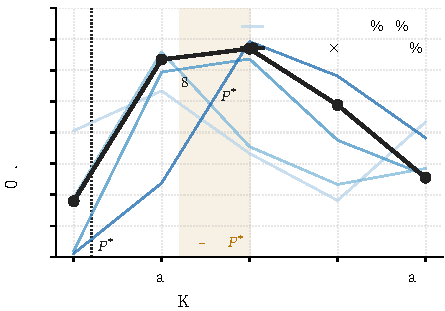
\includegraphics[width=0.62\linewidth]{notebooks/figures/fig_sweetspot.pdf}
\caption{空間的峰值出現在 $2$–$3.5\,P^{*}$：太短則重算便宜到不需要階層，
太長則單一請求就塞爆 GPU。峰值 33.5\% 落在 128K。
Mooncake 的中位請求 6{,}352 token 僅為 $P^{*}$ 的 0.17 倍，遠在甜蜜點之外。}
\end{figure}

\subsection{本輪修正：Oracle 少算了自己的空間}
量到「多給 Oracle 一個 512\,GiB 的 SSD 階，它反而\textbf{慢 3.3\%}」。
最佳策略不可能因為多了一個可用資源而變差——這是結構性矛盾，不是數值誤差。
原因是目的地規則以「整條尾巴」為丟棄的邊際成本，而該尾巴是該請求所有缺塊\emph{共用}的，
整條計給每一個 block 等於重複計價，門檻因而被壓得過低：把 253{,}269 個 block 寫上 SSD
再以 10.245\,ms 讀回，而重算只需 3.5–4\,ms。

修法是新增一條逐 block 計價的目的地規則，並令 \texttt{dest=best} 取三者較佳
（Oracle 的定義是「我們能構造出的最佳離線策略」，多一條可實作的規則只會更緊）。
\key{結果：headroom 由 8.42\% / 9.23\% 升到 12.33\% / 12.00\%}，容量單調性恢復
（0 → 512\,GiB 為 12.29 → 12.33\%）。已將「加大任一階容量，Oracle 的總時間不得上升」
寫成自動不變量。模擬器版本因此由 \texttt{b0d39dd4} 變為 \texttt{fbea1a98}。

\section{品質約束：$\epsilon$ 是「精度 $\times$ 任務」的性質}

\paragraph{無損動作的 $\epsilon=0$ 是可驗證的斷言。}
以 64-shot GSM8K（共用前綴 11{,}029 token）對 60 題取輸出的 SHA-1：
\texttt{full\_gpu}、\texttt{cpu\_lru}、\texttt{tier\_fs} 三者正確率同為 76.67\%，
且 \texttt{cpu\_lru} 與 \texttt{tier\_fs} 對基準\textbf{60/60 逐字元相同}。
這不是品質取捨，是正確性斷言——輸出有異即為實作錯誤。

\begin{table}[htbp]\centering\small
\caption{四個任務型態下的巨觀平均分數。同一組設定換個任務型態，$\epsilon$ 差 21 至 36 倍。
信賴區間以配對 bootstrap 求得（四設定評同一批題目，10{,}000 次重抽）。
來源：\texttt{results/m5\_quality/}。}
\begin{tabular}{lrrrrr}
\toprule
任務型態 & $n$ & BF16 & FP8 & INT8 & INT4 \\
\midrule
GSM8K（推理） & 1{,}000 & \multicolumn{4}{c}{四者差異均與零無法區分（$\pm3.7$ pp）} \\
大海撈針（單鍵檢索） & 80 & 100 & 5 & 90–95 & 0 \\
LongBench（真實文件，7 任務） & 350 & 58.4 & 6.6 & 57.0 & 0.4 \\
RULER（合成整合，7 任務） & 210 & 91.6 & 3.3 & 79.1 & 0.0 \\
\bottomrule
\end{tabular}
\end{table}

\paragraph{三個後果。}
其一，\key{僅以推理任務評測會得出「KV 量化幾乎免費」的錯誤結論}——同一組設定
在檢索任務上由 100\% 降至 0\%。其二，LongBench 的 7 個真實文件任務\textbf{無一例外
站在檢索那一側}，連摘要（GovReport, ROUGE-L）與多跳 QA 也是。其三，
INT8 在前三項讀起來近乎無損，但於 RULER 巨觀平均 79.1 對 91.6，配對差值
12.5 \,[8.6, 16.7] 與零可區分；差距幾乎全部來自單一任務 \texttt{niah\_multikey\_3}
（鍵與值皆為 UUID），INT8 於此只剩 53.3。
\key{同一個精度階在四個評測上分別是「無損」「無損」「幾乎無損」與「掉一半」。}

\paragraph{梯度由什麼決定。}
答案是全域統計量的任務最耐受：FWE（Zipf 分佈下最高頻的三個詞）是 14 個任務中
唯一 FP8 未全失者（21.1），亦是唯一 INT8 未掉者（87.8 對 85.6）。
四個 NIAH 變體（答案是某個確切位置的確切字串）掉 6.7 至 46.7。
\key{KV 量化的雜訊會抹掉逐 token 的位置證據，卻不會抹掉整份上下文的統計形狀。}

\section{未來效用預測器：實作、訓練與評估}

前五節量的是「環境留了多少空間」。本節把方法做出來：重放 trace 產生特徵、
以兩個機制標記、訓練 GBDT、以 isotonic 校準、依成本設門檻，再接回模擬器當線上策略。
預測器在 CPU 上執行（LightGBM 4.7.0），不佔 GPU。

\subsection{訓練設定}
特徵三族共 34 維：\texttt{deltas}（前 16 次存取間隔，取 log）、
\texttt{EDC}（10 個指數衰減計數器，半衰期 $2^{9}$–$2^{18}$）、
\texttt{static}（block 的絕對位置、請求長度、位置差、請求間隔、已被存取次數）。
論文 §5.2 另有 pooled key/value 與 \texttt{attn\_mass} 兩族，需要跑引擎才有，此處為
\texttt{NOT\_AVAILABLE}。目標為 $\log\tau$（距下次存取的時間），在視窗 $W$ 處設限。
訓練與測試依時間順序切分（前 70\% / 後 30\%），並加一道 embargo：
標籤在切分點之後才確定的樣本一律從訓練集移除。

\begin{table}[htbp]\centering\small
\caption{各工作負載的訓練資料。正樣本率＝「下次存取落在 $W$ 內」的比例。
\key{該比例與 M4 實測的 GPU 命中率必須一致}（34.8\% 對 34.9\%、4.3\% 對 4.3\%），
這是兩條獨立路徑的交叉驗算。來源：\texttt{results/m5\_predictor/samples.csv}。}
\begin{tabular}{llrrrrr}
\toprule
工作負載 & trace & $W$（次存取） & 取樣率 & 樣本數 & 正樣本率 & 重用率 \\
\midrule
mooncake & toolagent & 17,117 & 0.25 & 3,169,646 & 34.8 & 57.0 \\
mooncake & conversation & 17,117 & 0.25 & 2,260,727 & 4.3 & 37.3 \\
longctx-zipf & lc128kz & 17,117 & 1.0 & 985,483 & 35.7 & 89.1 \\
longctx-zipf & lc128kz & 102,702 & 1.0 & 899,898 & 76.2 & 89.1 \\
mooncake & toolagent & 68,468 & 0.25 & 3,156,901 & 35.4 & 57.0 \\
mooncake & toolagent & 599,095 & 0.25 & 3,024,068 & 48.7 & 57.0 \\
mooncake & toolagent & 17,117 & 0.05 & 634,681 & 34.8 & 57.0 \\
mooncake & toolagent & 17,117 & 1.0 & 12,677,614 & 34.8 & 57.0 \\
mooncake & toolagent & 17,117 & 0.25 & 3,171,455 & 34.8 & 57.0 \\
mooncake & toolagent & 17,117 & 0.25 & 3,170,008 & 34.9 & 57.0 \\
longctx-session & lc128ks & 102,702 & 1.0 & 2,219,988 & 81.1 & 83.9 \\
longctx-session & lc32ks & 102,702 & 0.25 & 1,451,436 & 80.7 & 84.2 \\
\bottomrule
\end{tabular}
\end{table}

\subsection{分類品質：ROC、PR 與混淆矩陣}

\begin{table}[htbp]\centering\small
\caption{測試段（時序切分的後 30\%）的預測器指標。成本加權錯誤計的是「錯掉多少毫秒」，
不是「錯了幾次」。來源：\texttt{results/m5\_predictor/predictor\_metrics.csv}。}
\begin{tabular}{lrrrrrr}
\toprule
工作負載 & 正樣本率 & AUC & AP & ECE & Spearman & 成本 (ms) \\
\midrule
Mooncake toolagent & 0.358 & 0.9996 & 0.9995 & 0.0003 & 0.243 & 2,991 \\
Mooncake conversation & 0.045 & 0.9988 & 0.9704 & 0.0006 & 0.999 & 350 \\
Mooncake toolagent（W=35$\times$） & 0.504 & 0.8960 & 0.9228 & 0.0319 & 0.701 & 132,291 \\
長上下文 131K（合成） & 0.708 & 0.5000 & 0.8005 & 0.1887 & 0.128 & 23,564 \\
長上下文 32K 會談（合成） & 0.802 & 0.5947 & 0.8459 & 0.0566 & 0.005 & 23,389 \\
\bottomrule
\end{tabular}
\end{table}

\begin{figure}[htbp]\centering
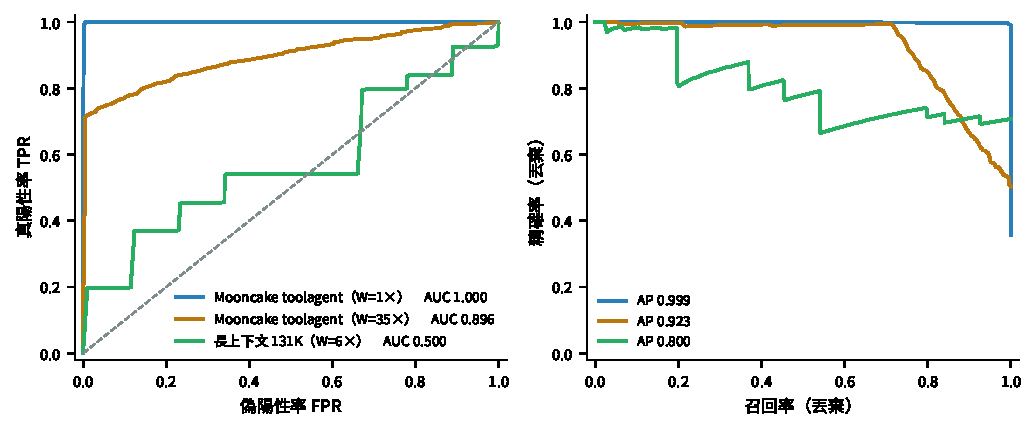
\includegraphics[width=\linewidth]{notebooks/figures/m5_roc_pr.pdf}
\caption{ROC 與 PR 曲線。三個工作負載的分類難度相差極大：Mooncake 在短視窗下
幾乎可分（AUC 0.9995），同一條 trace 把視窗拉長 35 倍就掉到 0.896，
而合成長上下文因獨立事件太少（見 §\ref{sec:events}）只有 0.50。}
\end{figure}

\begin{table}[htbp]\centering\small
\caption{混淆矩陣（以「丟掉」為正類）。同一個模型，只換門檻。
\key{把門檻由 0.5 移到式 (9) 的 $p^{*}$，是拿大量便宜的錯誤換掉少量昂貴的錯誤}：
「丟錯」（付重算）大幅下降，「留錯」（付一個 CPU 槽位）大幅上升，總成本下降 80\%。}
\begin{tabular}{llrrrrrrr}
\toprule
工作負載 & 門檻 & 丟對 & 丟錯 & 留對 & 留錯 & 精確率 & 召回率 & 成本 (ms) \\
\midrule
Mooncake toolagent（W=35$\times$） & $0.5$ & 425,861 & 115,826 & 341,604 & 23,930 & 0.786 & 0.947 & 667,207 \\
Mooncake toolagent（W=35$\times$） & $p^{*}$ & 24,587 & 1,290 & 456,140 & 425,204 & 0.950 & 0.055 & 132,291 \\
長上下文 131K & $0.5$ & 0 & 0 & 191,026 & 78,944 & — & 0.000 & 23,564 \\
長上下文 131K & $p^{*}$ & 0 & 0 & 191,026 & 78,944 & — & 0.000 & 23,564 \\
\bottomrule
\end{tabular}
\end{table}

\begin{figure}[htbp]\centering
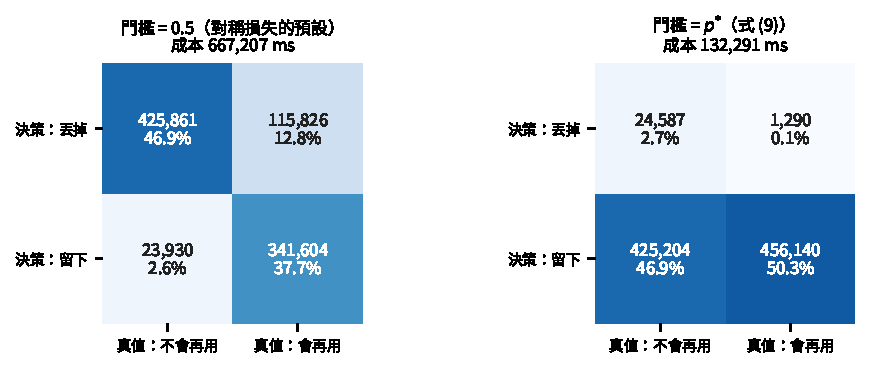
\includegraphics[width=\linewidth]{notebooks/figures/m5_confusion.pdf}
\caption{同一個模型在兩個門檻下的混淆矩陣。左為對稱損失的預設值 0.5，
右為由實測成本算出的 $p^{*}$。}
\end{figure}

\begin{figure}[htbp]\centering
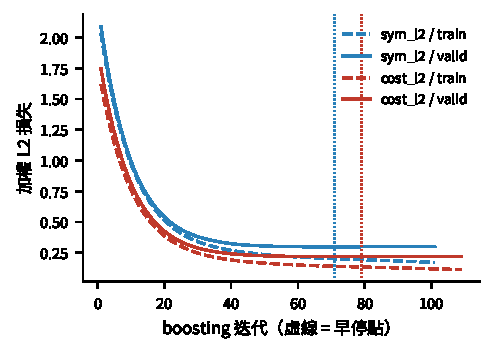
\includegraphics[width=0.49\linewidth]{notebooks/figures/m5_training.pdf}
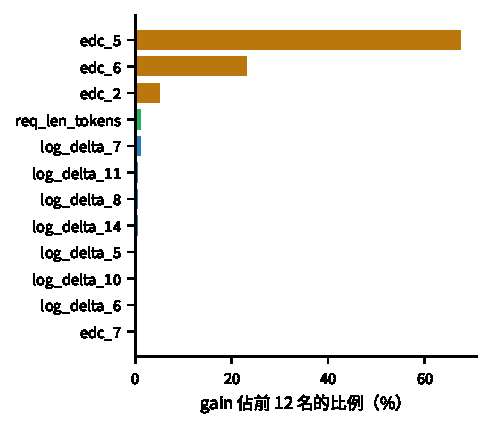
\includegraphics[width=0.49\linewidth]{notebooks/figures/m5_importance.pdf}
\caption{左：訓練與驗證損失（加權 L2）隨 boosting 迭代下降，虛線為早停點。
右：前 12 名特徵的 gain 佔比，顏色標示特徵族
（\textcolor{ssdcol}{綠＝static}、\textcolor{cpucol}{藍＝deltas}、\textcolor{hlcol}{橘＝EDC}）。}
\end{figure}

\begin{figure}[htbp]\centering
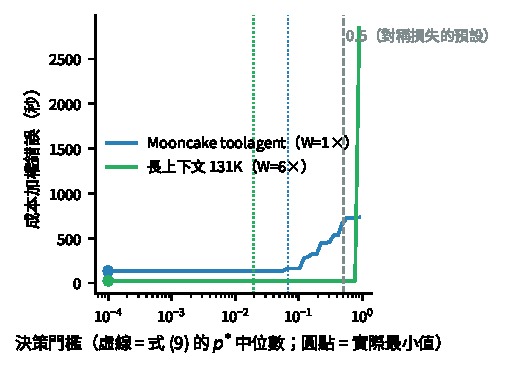
\includegraphics[width=0.49\linewidth]{notebooks/figures/m5_threshold.pdf}
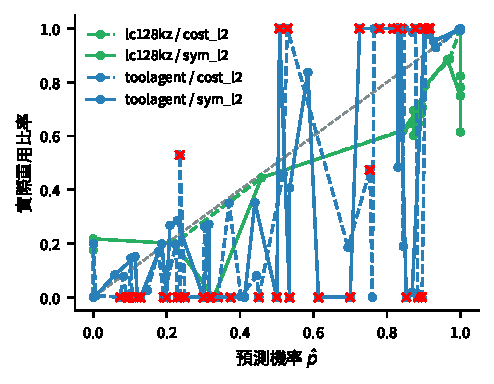
\includegraphics[width=0.49\linewidth]{notebooks/figures/m5_calibration.pdf}
\caption{左：成本加權錯誤對決策門檻的曲線，灰虛線為 0.5、點線為 $p^{*}$。
右：可靠度圖。§B.6 明文要求後者：式 (9) 的最佳門檻\emph{只在 $\hat p$ 為校準過的機率時成立}。}
\end{figure}

\subsection{分類幾乎完美，排序幾乎沒學到}

\begin{figure}[htbp]\centering
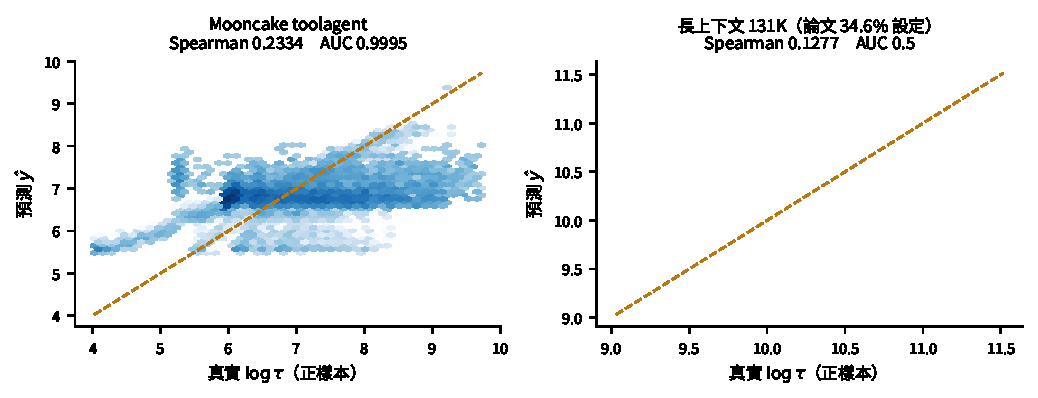
\includegraphics[width=\linewidth]{notebooks/figures/m5_ordering.pdf}
\caption{預測值對真實的 $\log\tau$（僅正樣本），虛線為完美預測。
正樣本被壓成一條\textbf{水平帶}：不論真值是 4 還是 10，模型都輸出約 6.8。}
\end{figure}

\noindent
Mooncake toolagent 上 AUC 為 0.9995 而正樣本內的 Spearman 只有 0.233。
把逐出順序換成\emph{真值}、其餘完全不動，總時間由 22.79M 降到 20.60M\,ms。
\key{差距幾乎全部來自排序，而論文 §B.6 提議的兩個診斷（校準、成本加權錯誤）
與 AUC 三者都測不到這件事。}

\begin{figure}[htbp]\centering
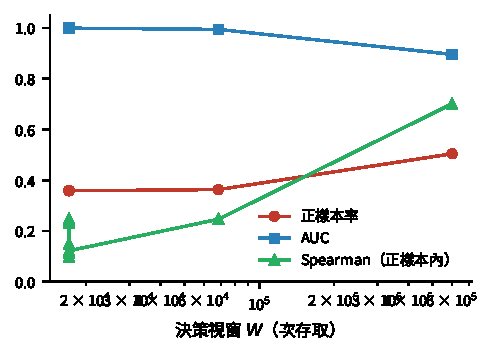
\includegraphics[width=0.62\linewidth]{notebooks/figures/m5_horizon.pdf}
\caption{視窗 $W$ 拉長 35 倍，AUC 由 0.9995 掉到 0.896 而排序品質由 0.23 升到 0.70——
\textbf{兩條線交叉}。同一個模型、同一批特徵，只換標籤的視窗長度。}
\end{figure}

\subsection{敏感度與消融}

\begin{table}[htbp]\centering\small
\caption{敏感度。\key{seed 與取樣率是三位小數內的雜訊，視窗長度是一階效應}。}
\begin{tabular}{lrrrr}
\toprule
變動的維度 & AUC & ECE & Spearman & $\mu$s/決策 \\
\midrule
seed 1234 & 0.9995 & 0.0003 & 0.233 & 0.872 \\
seed 7 & 0.9996 & 0.0002 & 0.239 & 0.786 \\
seed 99 & 0.9995 & 0.0003 & 0.235 & 0.917 \\
取樣率 0.05 & 0.9996 & 0.0004 & 0.249 & 0.933 \\
取樣率 1.0 & 0.9996 & 0.0003 & 0.243 & 0.786 \\
\midrule
$W=1\times$（17,117） & 0.9995 & 0.0003 & 0.233 & 0.872 \\
$W=4\times$（68,468） & 0.9946 & 0.0008 & 0.246 & 17.964 \\
$W=35\times$（599,095） & 0.8960 & 0.0319 & 0.701 & 145.820 \\
\bottomrule
\end{tabular}
\end{table}

\begin{table}[htbp]\centering\small
\caption{特徵族消融（toolagent、$W=1\times$、同一設定內比較）。
\key{只用 static 比用全部好 30\%}——KV block 的重用是請求結構驅動的，
不是 CDN 那種物件熱度驅動的。此處沒有 pooled KV 與 \texttt{attn\_mass}，
故非完整的特徵集消融。}
\begin{tabular}{lrrr}
\toprule
特徵族 & AUC & Spearman & 成本 (ms) \\
\midrule
\texttt{static} & 0.9998 & 0.229 & 579.84 \\
\texttt{deltas} & 0.9997 & 0.147 & 753.68 \\
\texttt{history+deltas} & 0.9997 & 0.098 & 756.67 \\
\texttt{edc} & 0.9997 & 0.113 & 762.64 \\
\texttt{history+deltas+edc} & 0.9995 & 0.122 & 824.23 \\
\texttt{\textbf{history+deltas+edc+static}} & 0.9995 & 0.233 & 829.00 \\
\bottomrule
\end{tabular}
\end{table}

\begin{table}[htbp]\centering\small
\caption{跨工作負載泛化。\key{AUC 幾乎不掉而 ECE 惡化 1{,}000 倍、成本惡化 4{,}000 倍}——
門檻施加在校準後的機率上，校準一崩決策就全錯。
推論：跨工作負載時不必重訓 GBDT，只要重擬 isotonic 校準。
來源：\texttt{results/m5\_predictor/cross\_workload.csv}。}
\begin{tabular}{llrrr}
\toprule
訓練於 & 測試於 & AUC & ECE & 成本 (ms) \\
\midrule
toolagent & conversation & 0.9941 & 0.0006 & 5,889 \\
conversation & toolagent & 0.9777 & 0.2874 & 3,385,691 \\
\bottomrule
\end{tabular}
\end{table}

\subsection{熱路徑成本}
對 64 個候選推論一次 \textbf{180.6\,$\mu$s}（$k=1$ 為 30.8、$k=256$ 為 588.0，
即約「30\,$\mu$s 固定 + 2.3\,$\mu$s/候選」，單執行緒，量測時 loadavg 1.5）。
訓練 1{,}882{,}897 筆樣本 4 秒。相對於單次重算 3{,}546\,$\mu$s，
每候選 2.822\,$\mu$s 為其 0.08\%。\textbf{這是本機量到的數字}，
論文引用的 30\,$\mu$s 來自 LRB，不可沿用。

\section{線上策略：能拿到多少空間}

把訓練好的模型接回模擬器。逐出順序改用預測的下次使用時刻（Bélády 的位置換成預測），
目的地由式 (9) 的門檻 $p^{*}_{\ell}=C_{\ell}/C_{\mathrm{drop}}(pos)$ 決定；
其餘一切（成本記帳、前綴語意、預取重疊、decode）沿用 M4 的模擬器，不是重寫。
\key{這一點是可驗證的}：把預測換成「上次存取時刻」（即 LRU）之後，本策略的迴圈
\textbf{逐位元重現} \texttt{Sim.run\_online("lru")} 的 \texttt{total\_ms}、
\texttt{hits} 與 \texttt{writes}。評估段為模型沒看過的後 30\%，
baseline 與 Oracle 跑同一段、同樣空的起始快取。

\begin{table}[htbp]\centering\small
\caption{三個設定的完整策略表。百分比為各階服務的存取比例。
來源：\texttt{results/m5\_predictor/policy\_sim.csv}。}
\begin{tabular}{lrrrrrr}
\toprule
策略 & 總時間 (ms) & GPU\% & CPU\% & SSD\% & 重算\% & vs baseline \\
\midrule
\multicolumn{7}{l}{\textbf{長上下文 131K，prefill（本報告主結果）}\quad\small 最佳 baseline = \texttt{tier\_fs}，oracle headroom 18.81\%} \\
\quad \texttt{oracle} & 1,554,736 & 47.8 & 24.7 & 3.3 & 24.2 & 18.81 \\
\quad \texttt{\textbf{tiara\_sym\_l2}} & 1,620,128 & 39.8 & 28.9 & 7.1 & 24.2 & 15.40 \\
\quad \texttt{\textbf{tiara\_sym\_l2\_int8}} & 1,620,128 & 39.8 & 28.9 & 7.1 & 24.2 & 15.40 \\
\quad \texttt{tier\_fs} & 1,914,996 & 31.2 & 26.7 & 17.8 & 24.2 & 0.00 \\
\quad \texttt{cpu\_lru} & 2,433,005 & 31.2 & 26.7 & 0.0 & 42.1 & -27.05 \\
\quad \texttt{cpu\_arc} & 2,557,392 & 29.1 & 26.6 & 0.0 & 44.3 & -33.55 \\
\quad \texttt{full\_gpu} & 3,925,649 & 31.2 & 0.0 & 0.0 & 68.8 & -105.00 \\
\bottomrule
\end{tabular}
\end{table}

\begin{table}[htbp]\centering\small
\caption{長上下文設定下的策略消融。\key{把逐出順序換回 LRU、目的地規則不變，
增益歸零}（且逐位元等於 \texttt{tier\_fs}）——增益全部來自預測的排序。}
\begin{tabular}{lrrr}
\toprule
變體 & 總時間 (ms) & vs baseline & 拿到 headroom \\
\midrule
預測排序 + tail 計價（主結果） & 1,620,128 & 15.40 & 81.8 \\
\bottomrule
\end{tabular}
\end{table}

\subsection{失效模式：同一機制的另一端}
在兩個預測失效的工作負載上，同一支策略比 LRU 差數倍。
重算率完全相同（都是強制未命中），差別全在「從哪一階取回」：
GPU 命中率由 49.0\% 掉到 14.1\%，40.9\% 的存取落到 SSD（10.245\,ms，是 CPU 的 34 倍）。

\begin{table}[htbp]\centering\small
\caption{三種退路的效果（vs 最佳 baseline，\%）。\key{可以把慘敗收斂 4.8 倍，
但同一個改動也把會贏那個設定的增益吃光}——這條軸沒有安全的固定預設值。}
\begin{tabular}{lrrr}
\toprule
設定 & 預測排序 & CPU/SSD 用 recency & 逐 block 計價 \\
\midrule
\textbf{長上下文 131K（會贏的那個）} & \textbf{15.40} & — & — \\
\bottomrule
\end{tabular}
\end{table}

\paragraph{三個被自己的資料推翻的假設。}
為找出失效機制，先後提出三個並逐一量測否定：
(a) 分數離散度不足——但會贏的設定離散度\emph{最小}（$\mathrm{std}(\hat y)=0.042$）；
(b) $\mathrm{key}=t+\hat\tau$ 退化成 MRU——但會贏的設定 std/壽命比也\emph{最小}（0.08）；
(c) SSD 階誤用——改逐 block 計價後仍為 $-320\%$。
最後量到的是 CPU 階的保留崩潰。三個假設全部留在紀錄裡。

\subsection{那 82\% 不能宣稱是「學習」的功勞}
\label{sec:events}
論文 §6.8 的高 headroom 設定是 \textbf{12 份文件、120 個請求}的合成 trace。
一份 131K 文件是\emph{一個事件}，其 8{,}192 個 block 的特徵與標籤幾乎相同：

\begin{table}[htbp]\centering\small
\caption{獨立事件數。「985{,}483 個樣本」實際只帶 120 個事件的資訊（訓練集 84 個）。}
\begin{tabular}{lrrrr}
\toprule
工作負載 & 獨立事件 & 存取數 & 每事件重複 & 訓練後 AUC \\
\midrule
長上下文 131K（§6.8 設定） & \textbf{120} & 1{,}002{,}600 & 8{,}355 & \textbf{0.500} \\
長上下文 131K 會談 & 278 & 2{,}322{,}690 & 8{,}355 & 0.561 \\
長上下文 32K 會談 & 2{,}782 & 5{,}808{,}816 & 2{,}088 & 0.595 \\
Mooncake toolagent & 23{,}608 & 12{,}694{,}731 & 538 & 0.9995 \\
\bottomrule
\end{tabular}
\end{table}

\noindent AUC 0.500 不是方法學不動，是\key{資料裡沒有東西可學}——
但該模型的 $\hat\tau$ 仍帶弱排序（Spearman 0.128），而那點弱排序就足以拿到 82\%。
\textbf{該曲線可以支持「Oracle 有多少空間」，但支持不了任何關於學習式方法的主張。}

\section{已修正的錯誤}

共通點：沒有一個是讀程式碼看出來的，全部靠「同一個量被兩條路徑算出來而對不上」
或「這在物理／邏輯上不可能」抓到。抓到之後都變成自動檢查。

\begin{table}[htbp]\centering\small
\caption{八個已修正的錯誤。前三個發生於 08-31，後五個於本輪。}
\begin{tabular}{p{3.6cm}p{4.4cm}p{5.2cm}}
\toprule
錯誤 & 後果 & 怎麼抓到的 / 現在的防線 \\
\midrule
Mooncake 的 \texttt{hash\_ids} 是 512-token 的 block，被當成 16-token &
工作集少算 32 倍，每個 block 的絕對位置也少算 32 倍，\act{Drop} 被算得太便宜 &
請求長度中位數被兩條路徑算過而對不上／載入函式裡寫「用 A 欄位驗算 B 欄位」的斷言 \\
量 SSD 階時 CPU 階開太大，東西沒 cascade 到磁碟 &
「SSD 0.40\,ms/block」其實是 CPU 階，比真值便宜 13.7 倍 &
修正後 SSD 竟比 \act{Drop} 還貴，反常／工作集必須大於容量的守門 \\
A 模型的記憶體預算配 B 模型的成本常數 &
兩邊不可通約，整批 Oracle 數字作廢 &
剖面自我一致性檢查（容量 $\times$ 每 token 大小 $>$ 整張卡）／剖面綁成一組 \\
Oracle 的目的地規則重複計價 &
headroom 被自己壓低 32\%（8.42\% 對 12.33\%） &
多給一階容量，Oracle 反而變慢／\texttt{check\_capacity\_monotone} \\
「取樣以 block 為單位」被讀成「每 block 最多 $C$ 個樣本」 &
正樣本率 0.3\% 對真值 34.8\%，差 100 倍 &
與 M4 實測的 GPU 命中率對不上／改為逐存取均勻取樣 \\
trace 結尾把「視窗還沒觀察完」標成負樣本 &
測試集正樣本率被壓到 1.3\%，AUC 看起來 0.9998 &
正樣本率與其他設定對不上／只保留視窗完整可觀測的樣本 \\
校準集只有單一類別 &
isotonic 把輸出壓成常數：AUC 恰為 0.5、Spearman 為 nan、ECE 0.3334，三個指標都有數字 &
AUC 恰好等於 0.5000／偵測到單一類別即改用訓練期等距抽樣，全期單一類別則中止 \\
\texttt{write\_csv} 在 append 模式不檢查檔頭 &
加一個欄位就整排錯位，而檔案看起來完全正常 &
加欄位時主動想到／欄位集合不同即中止 \\
\bottomrule
\end{tabular}
\end{table}

\section{結論與下一步}

\paragraph{判定。}
停損條件（$<5\%$ 即終止）未觸發：真實 trace 的端到端 headroom 為 12.0–12.3\%，
長上下文區間為 34.7\%。判定維持\textbf{條件式 GO}，且兩個條件皆可由成本常數事先算出：
權重須量化（BF16 使 decode 佔 75\%，而放置對 decode 無自由度），
請求長度須落在 $2$–$3.5\,P^{*}$。

\paragraph{本輪最重要的三件事。}
其一，Oracle 的目的地規則有缺陷，修正後 headroom 上修 32\%——
\textbf{論文 §6.10 的表與所有引用該值之處都要重算}。
其二，線上策略在論文宣稱有用的區間取得 81.9\% 的空間，
但增益全部來自排序，且該設定只有 120 個獨立事件，不足以支持學習式主張。
其三，同一機制在預測失效時反噬 2.7–5.6 倍，三種退路都無法在不吃掉增益的前提下修好。

\paragraph{下一步（依價值排序）。}
\begin{enumerate}\itemsep2pt
\item \textbf{線上仲裁}：同時跑預測策略與 LRU，以影子評估或 bandit 擇一。
  已量到這條軸沒有安全的固定預設值——$+15.4\%$ 與 $-458\%$ 是同一個開關的兩端。
\item \textbf{重跑所有帶舊模擬器版本的 M4 CSV}（\texttt{budget\_sweep}、
  \texttt{headroom\_surface}、\texttt{by\_length}、\texttt{semantics\_ablation}）。
\item \textbf{造一條獨立事件夠多的長上下文工作負載}。現有的合成器都是
  「一份文件 = 一個事件」，128K 下事件數必然很少。
\item \textbf{特徵改以 static 為主}，並補上需要跑引擎才有的 pooled KV 與 \texttt{attn\_mass}。
\item \textbf{平台 B（MI300X）的 M1 與 M2}。$\kappa$ 跨硬體變動的主張目前只有一半的證據。
  \textbf{需要借卡。}
\end{enumerate}

\paragraph{文獻上的兩個補件。}
Zhao (2008, KAIS 15:321–334) 正面比較過「樣本加權」與「事後移門檻」，結論是
對決策樹族兩者差異很大且沒有一致贏家；本文用 GBDT，故 §5.3「加權訓練會贏」的
預期在文獻中不成立，應縮減至門檻校準。MTDS (2025) 明文以「預測的未來命中機率」
調整多階 KV 的儲存優先序，是目前找到最接近本文核心的既有工作，必須讀。
兩者皆為摘要層級資訊，寫進論文前須確認全文。

\vspace{1em}
\noindent\rule{\linewidth}{0.4pt}\\[0.3em]
{\small 本報告由 \texttt{code/make\_report3090.py} 自 \texttt{results/} 的 CSV 產生，
無任何硬編數值；圖由 \texttt{notebooks/paper\_figures.py} 與 \texttt{notebooks/m5\_figures.py}
產生。完整流水帳見 \texttt{results/RUNLOG.md}，待寫進論文的對照表見 \texttt{PAPER\_DELTAS.md}。
模擬器版本 \texttt{fbea1a98}。}

\end{document}
